\documentclass[a4paper]{jsarticle}
\usepackage[dvipdfmx]{graphicx}
%
\usepackage{amsmath,amssymb}
\usepackage{bm}
\usepackage{graphicx}
\usepackage{ascmac}
%
\setlength{\textwidth}{\fullwidth}
\setlength{\textheight}{40\baselineskip}
\addtolength{\textheight}{\topskip}
\setlength{\voffset}{-0.2in}
\setlength{\topmargin}{0pt}
\setlength{\headheight}{0pt}
\setlength{\headsep}{0pt}
%
\newcommand{\divergence}{\mathrm{div}\,}  %ダイバージェンス
\newcommand{\grad}{\mathrm{grad}\,}  %グラディエント
\newcommand{\rot}{\mathrm{rot}\,}  %ローテーション
%
\title{計算科学レポート}
\author{吉田 順一}
\date{\today}
\begin{document}
\maketitle
%
%
\section{オブジェクト}
$40 \rm{cm}\times 40\rm{cm} \times 1\rm{cm} $の水を$100$個並べたものを作成した。
\begin{figure}[h]
\centering
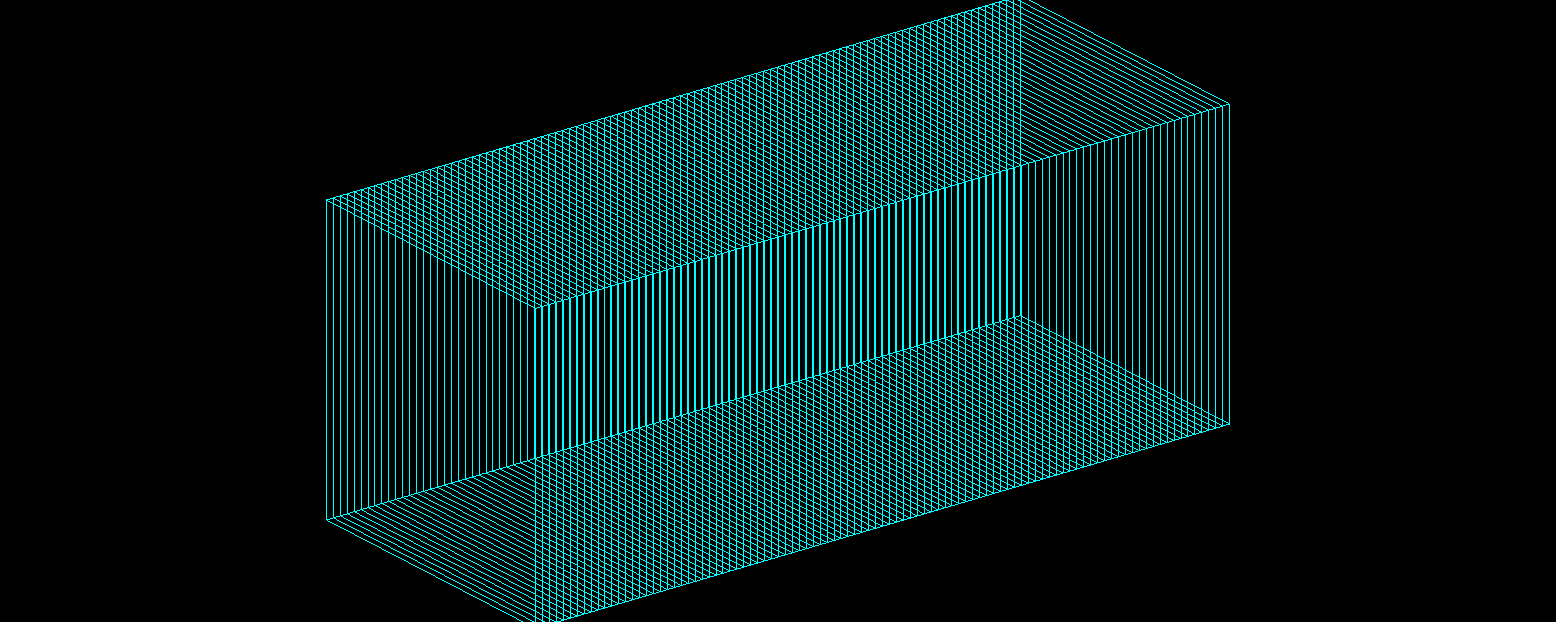
\includegraphics[width=10cm]{figure1.png}
\caption{オブジェクトの全体像}
\end{figure}

\section{実行結果}
陽子をz方向から入射した際に最初に当たる層から順に番号を0から99まで割り当てる。
水に付与されたエネルギーの大きさを各step毎に出力した。\\

\centering
\begin{tabular}[h]{c|c}
\hline
層番号&エネルギー損失(MeV) \\ \hline
0&5.67011\\
0&1.66172\\
1&5.61363\\
1&2.76592\\
2&4.88398\\
2&3.66544\\
3&4.15815\\
3&4.2686\\
3&0.836476\\
4&3.80582\\
4&3.56192\\
4&3.00461\\
5&3.3012\\
5&3.26144\\
5&2.75917\\
5&2.62731\\
5&0.467362\\
6&2.46696\\
6&2.58386\\
6&2.43178\\
6&2.19433\\
6&2.10997\\
6&2.05388\\
6&1.95708\\
6&1.13205\\
7&1.5786\\
7&1.62567\\
7&1.55982\\
7&1.44414\\
7&1.35253\\
7&1.35121\\
7&1.46308\\
7&1.27594\\
7&1.19589\\
7&1.09065\\
7&1.14837\\
7&1.06119\\
7&1.01598\\
7&0.966124\\
7&1.01479\\
7&1.0053\\
7&0.993065\\
7&1.03451\\
7&1.13804\\
7&1.26842\\
7&1.34884\\
7&0.402627\\
\end{tabular}\\
また、これらのデータを用いて各層におけるエネルギー損失をグラフにした。
\begin{figure}[h]
\centering
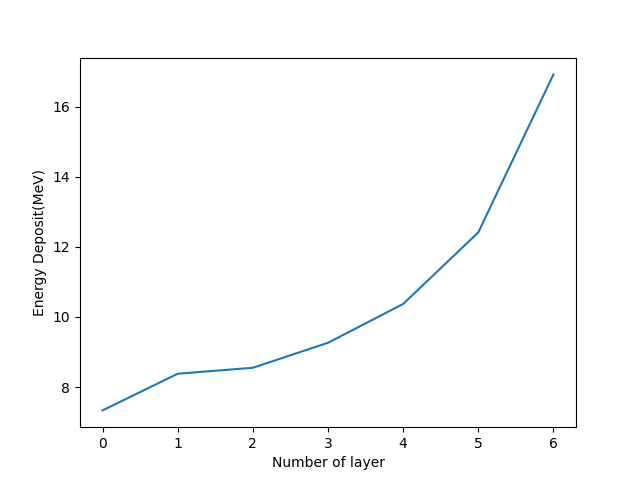
\includegraphics[width=10cm]{dataPlot.png}
\end{figure}\\
縦軸はエネルギー損失の大きさ、横軸は層の番号である。
\end{document}